% ================================================================
% Neural Demand Paper — CF Endogeneity Tables (auto-generated)
% N_RUNS = 5
% ================================================================

\begin{table}[htbp]
  \centering
  \caption{Control-Function RMSE — CES DGP (mean $\pm$ SE, 5 runs)}
  \label{tab:cf_endogeneity_ces}
  \begin{threeparttable}
  \begin{tabular}{lcccc}
    \toprule
    \textbf{Model} & $\rho=0.0$ & $\rho=0.3$ & $\rho=0.6$ & $\rho=0.9$ \\
    \midrule
    Neural Demand (static) & $0.00037 \pm 0.00002$ & $0.00035 \pm 0.00003$ & $0.00035 \pm 0.00003$ & $0.00039 \pm 0.00004$ \\
    Neural Demand (CF) & $0.00035 \pm 0.00002$ & $0.00037 \pm 0.00002$ & $0.00034 \pm 0.00004$ & $0.00034 \pm 0.00003$ \\
    Neural Demand (habit) & $0.00049 \pm 0.00005$ & $0.00047 \pm 0.00003$ & $0.00045 \pm 0.00001$ & $0.00050 \pm 0.00004$ \\
    Neural Demand (habit, CF) & $0.00046 \pm 0.00003$ & $0.00051 \pm 0.00002$ & $0.00049 \pm 0.00001$ & $0.00048 \pm 0.00003$ \\
    \bottomrule
  \end{tabular}
  \begin{tablenotes}\small
    \item RMSE evaluated against structural (IV-purged) demand at test prices.
    \item $\rho$ = endogeneity strength; $\rho=0$ is fully exogenous.
  \end{tablenotes}
  \end{threeparttable}
\end{table}

\begin{table}[htbp]
  \centering
  \caption{Control-Function RMSE — Habit DGP (mean $\pm$ SE, 5 runs)}
  \label{tab:cf_endogeneity_habit}
  \begin{threeparttable}
  \begin{tabular}{lcccc}
    \toprule
    \textbf{Model} & $\rho=0.0$ & $\rho=0.3$ & $\rho=0.6$ & $\rho=0.9$ \\
    \midrule
    Neural Demand (static) & $0.02239 \pm 0.00048$ & $0.02147 \pm 0.00053$ & $0.02310 \pm 0.00073$ & $0.02237 \pm 0.00088$ \\
    Neural Demand (CF) & $0.02286 \pm 0.00055$ & $0.02139 \pm 0.00047$ & $0.02316 \pm 0.00069$ & $0.02283 \pm 0.00102$ \\
    Neural Demand (habit) & $0.02053 \pm 0.00097$ & $0.01510 \pm 0.00042$ & $0.01669 \pm 0.00061$ & $0.01998 \pm 0.00118$ \\
    Neural Demand (habit, CF) & $0.02064 \pm 0.00086$ & $0.01521 \pm 0.00051$ & $0.01698 \pm 0.00061$ & $0.01966 \pm 0.00104$ \\
    \bottomrule
  \end{tabular}
  \begin{tablenotes}\small
    \item RMSE evaluated against structural (IV-purged) demand at test prices.
    \item $\rho$ = endogeneity strength; $\rho=0$ is fully exogenous.
  \end{tablenotes}
  \end{threeparttable}
\end{table}

\begin{figure}[htbp]
  \centering
  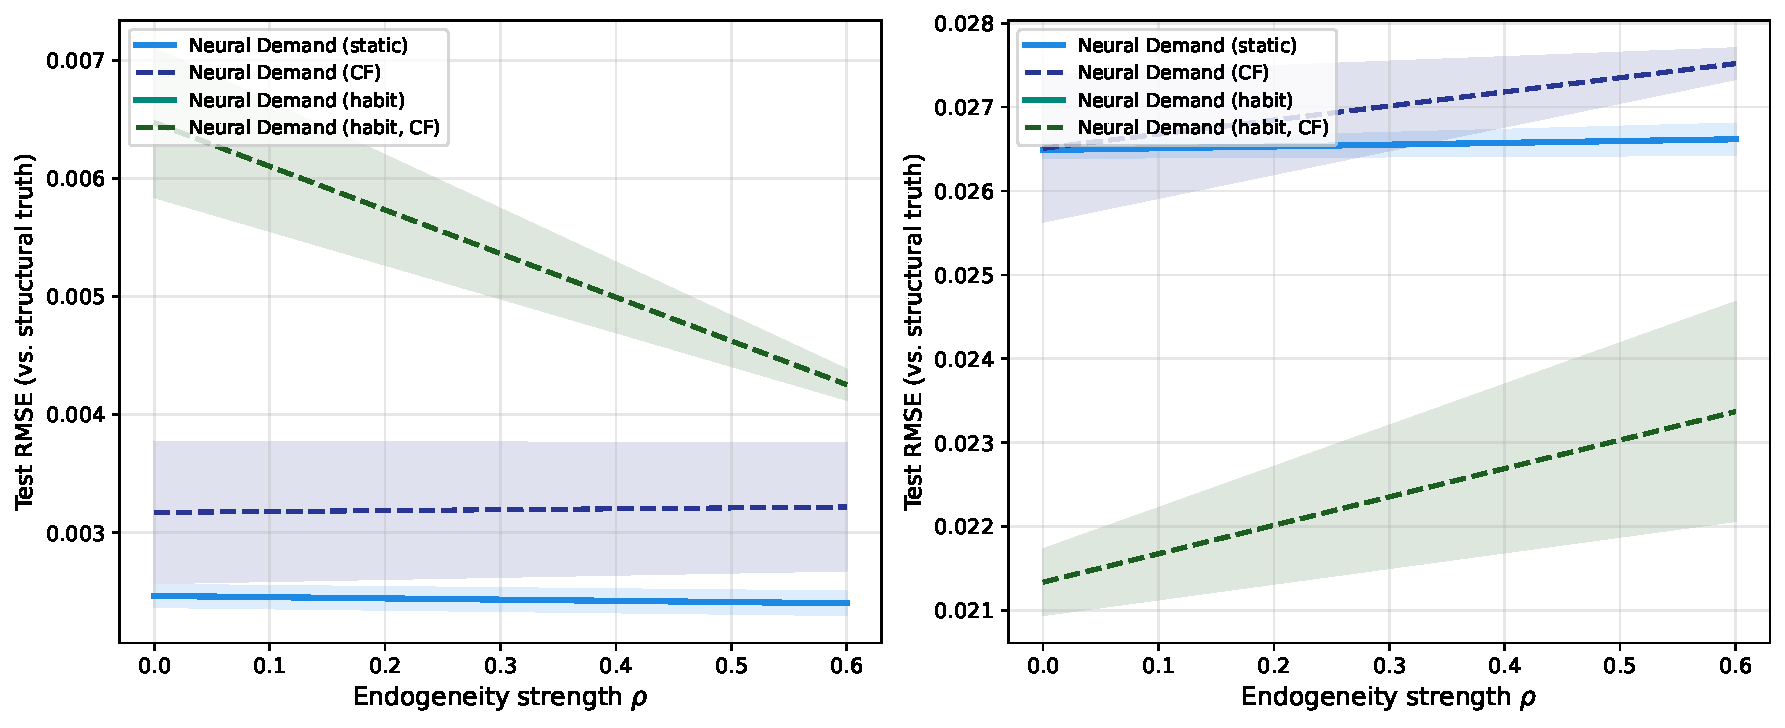
\includegraphics[width=0.85\linewidth]{results/neural_demand/simulations/figures/fig_cf_bias_reduction.pdf}
  \caption{RMSE vs.\ endogeneity strength $\rho$.  CF-corrected models (dashed) recover structural demand even at high $\rho$.}
  \label{fig:cf_bias_reduction}
\end{figure}

\begin{figure}[htbp]
  \centering
  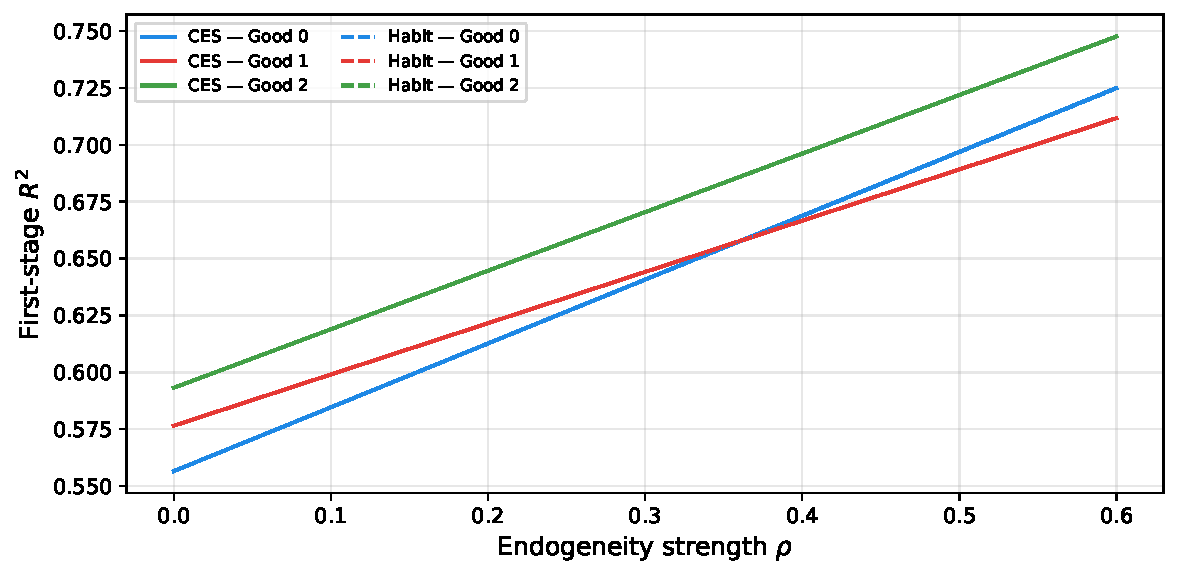
\includegraphics[width=0.85\linewidth]{results/neural_demand/simulations/figures/fig_cf_first_stage_rsq.pdf}
  \caption{First-stage $R^2$ for each good as a function of $\rho$, confirming instrument relevance.}
  \label{fig:cf_first_stage_rsq}
\end{figure}
